% vim:nojs:spelllang=en_au tw=76 sw=4 sts=4 fo+=awn fmr={-{,}-} et ts=8
\documentclass[11pt,a4paper]{report}
\usepackage{isabelle,isabellesym}

\usepackage{amssymb}
\usepackage[only,bigsqcap]{stmaryrd}

\usepackage{mathpartir}
\usepackage[margin=10mm,bottom=15mm]{geometry}
\usepackage[final]{graphicx}

% this should be the last package used
\usepackage{pdfsetup}

% urls in roman style, theory text in math-similar italics
\urlstyle{rm}
\isabellestyle{rm}

\begin{document}

\title{Loop freedom of the (untimed) AODV routing protocol}
\author{Timothy Bourke\thanks{Inria,
                              \'Ecole normale sup\'erieure,
                              and NICTA}
        \and
        Peter H\"ofner\thanks{NICTA
                              and Computer Science and Engineering, UNSW}}
\maketitle

\begin{abstract}
The Ad hoc On-demand Distance Vector (AODV) routing protocol~\cite{RFC3561} 
allows the nodes in a Mobile Ad hoc Network (MANET) or a Wireless Mesh 
Network (WMN) to know where to forward data packets. Such a protocol is 
`loop free' if it never leads to routing decisions that forward packets in 
circles.

This development mechanises an existing pen-and-paper proof of loop freedom 
of AODV~\cite{FehnkerEtAl:AWN:2013}.
The protocol is modelled in the Algebra of Wireless Networks (AWN),
which is the subject of an earlier paper~\cite{BourkeEtAl:MechAWN:2014} and 
mechanization~\cite{Bourke14}.
The proof relies on a novel compositional approach for lifting invariants to 
networks of nodes.

We exploit the mechanization to analyse several variants of AODV and show 
that Isabelle/HOL can re-establish most proof obligations automatically and 
identify exactly the steps that are no longer valid.
Each of the variants is essentially a modified copy of the main development.

Further documentation is available in~\cite{BourkevGlHof:ATVA:2014}.

\centering{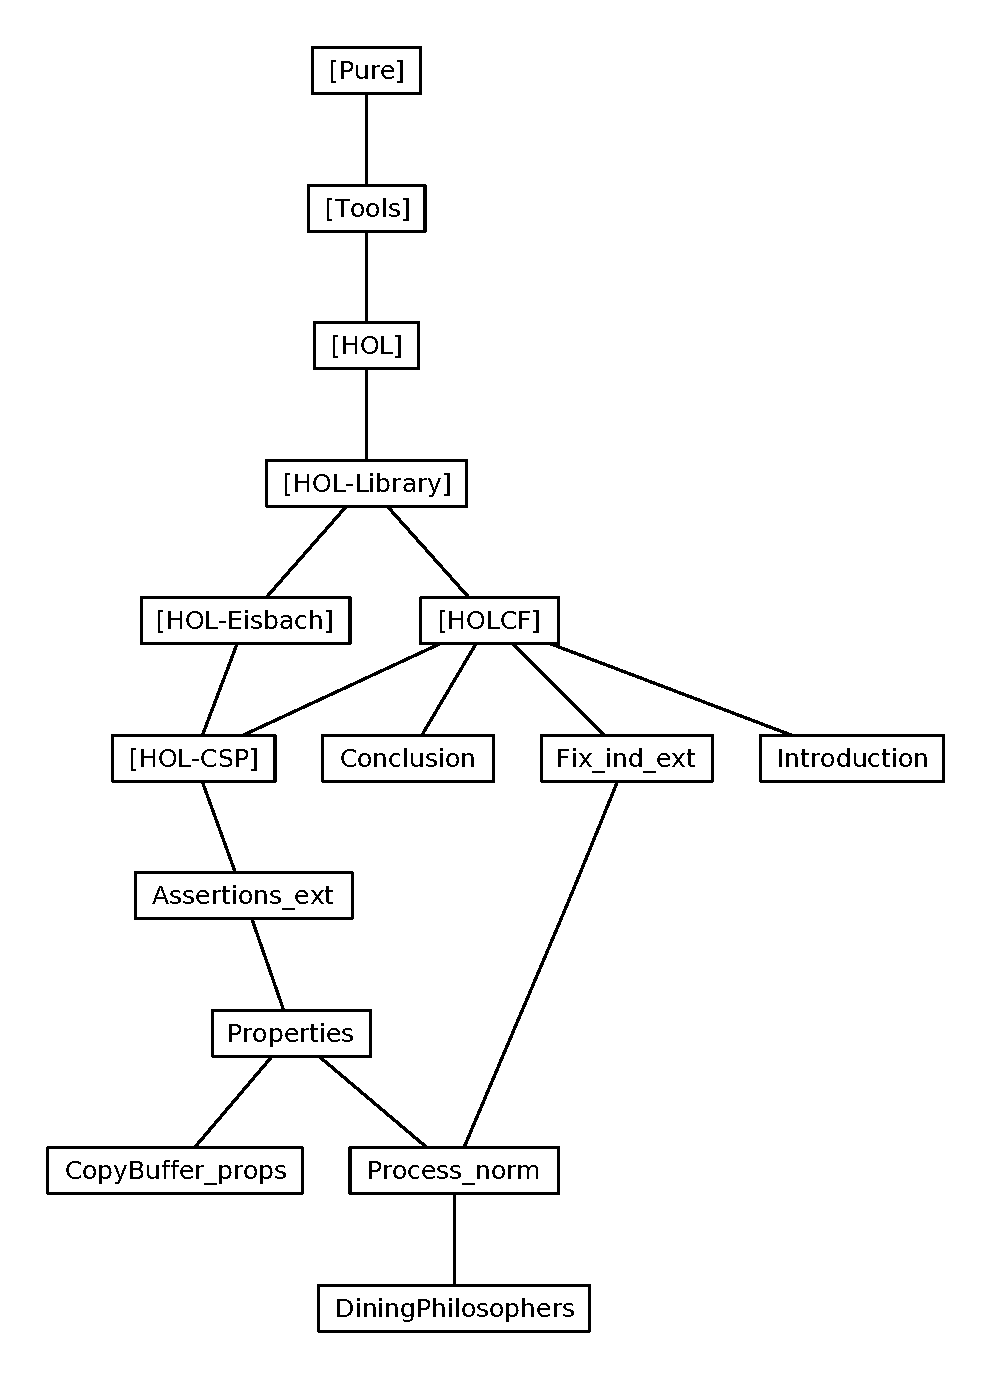
\includegraphics[width=\textwidth]{session_graph}}
\end{abstract}

\newpage
\tableofcontents

% sane default for proof documents
\parindent 0pt\parskip 0.5ex

% generated text of all theories
\newpage
\input{session}

% optional bibliography
\bibliographystyle{abbrv}
\bibliography{root}

\end{document}
